\documentclass[acmtog]{acmart}
\usepackage{graphicx}
\usepackage{float}
\usepackage{subfigure}
\usepackage{natbib}
\usepackage{listings}
\usepackage{bm}
\usepackage{amsmath}
\usepackage{algorithm}
\usepackage{algorithmic}



\definecolor{blve}{rgb}{0.3372549 , 0.61176471, 0.83921569}
\definecolor{gr33n}{rgb}{0.29019608, 0.7372549, 0.64705882}
\makeatletter
\lst@InstallKeywords k{class}{classstyle}\slshape{classstyle}{}ld
\makeatother
\lstset{language=C++,
	basicstyle=\ttfamily,
	keywordstyle=\color{blve}\ttfamily,
	stringstyle=\color{red}\ttfamily,
	commentstyle=\color{magenta}\ttfamily,
	morecomment=[l][\color{magenta}]{\#},
	classstyle = \bfseries\color{gr33n}, 
	tabsize=2
}
\lstset{basicstyle=\ttfamily}

% Title portion
\title{{Assignment 2 : Geometric Modeling}} 

\author{Name:\quad Bingnan Li\\ student number:\ 2020533092
\\email:\quad libn@shanghaitech.edu.cn}

% Document starts
\begin{document}
\maketitle

\vspace*{2 ex}
\setlength\parindent{2em}
\section{Introduction}
\begin{itemize}
\item Implemented evaluation function of Bézier curve with De Casteljau's algorithm.
\item Successfully constructed and drew Bézier surface (take Tea Party as an example)
\item Implemented adaptive mesh.
\item Implemented B-Spline mesh.
\end{itemize}
\section{Implementation Details}
\begin{enumerate}
	\setlength\parindent{2em}
	\item {\bf Bézier Curve:}
	\par With the recurrence formula
	\[P_{n,m} = (1-u)P_{n-1,m-1}+uP_{n-1,m}\]
	we can calculate the position of Bézier curve point with parameter $u$. Moreover, given that the line between $P_{n-1,m-1}$ and $P_{n-1,m}$ is tangent to Bézier where $P_{n,m}$ is in curve, we can calculate the normal vector of point $P_{n,m}$ by calculating $P_{n-1,m-1}-P_{n-1,m}$.
	\par {\it Pseudocode:}
	\begin{algorithm} 
		\caption{evaluate Bézier Curve} 
		% \label{alg3} 
		\begin{algorithmic}
			\STATE input: array $P[0:n]$ and real number $u$ in $[0,1]$
			\STATE output: position and normal on curve
			\FOR{$i:=0\to n$}
			\STATE Q[i]=P[i]
			\ENDFOR
			\FOR{$k:=1\to n$}
				\FOR{$i:=0\to n-k$}
					\IF{$i==n-k$}
						\STATE $normal:= Q[i]-Q[i+1]$ 
					\ENDIF
				\STATE $Q[i]=(1-u)Q[i]+uQ[i+1]$
				\ENDFOR
			\ENDFOR
			\RETURN Q[0], normal
		\end{algorithmic} 
	\end{algorithm}
	\item {\bf Bézier surface:}
	\begin{enumerate}
		\setlength\parindent{2em}
		\item {\bf Evaluation:}
		\par We can get the position of point with parameters $u,v$ by evaluating points along u direction with parameter $u$ and utilize those new points as new control points and evaluate the final point at parameter $v$.
		\par As for normal vector, we can perform the procedure above twice but in different orders. Namely, in the first turn, we evaluate the points with order $u,v$ and get corresponding normal vector along v direction. Then we perform the procedure in $v,u$ direction and get the corresponding normal vector. Lastly, we calculate the cross product of those two normal vector in order to get the normal vector of Bézier surface.  
		\par {\it Pseudocode:}
		\begin{algorithm} 
			\caption{evaluate Bézier surface} 
			% \label{alg3} 
			\begin{algorithmic}
				\STATE input: 2-d array $P[0:n][0:m]$ and real numbers $u,v$ in $[0,1]^2$
				\STATE output: position and normal on surface
				\FOR{$i:=0\to n$}
					\FOR{$j:=0\to m$}
						\STATE M[i][j] = P[i][j]
						\STATE N[j][i] = P[i][j]
					\ENDFOR
				\ENDFOR
				\FOR{$i:=0\to n$}
					\STATE line add $evaluate(M[i],u)$
				\ENDFOR
				\STATE $position, normal_1 = evaluate(line, v)$
				\FOR{$i:=0\to m$}
					\STATE line add $evaluate(N[i],v)$
				\ENDFOR
				\STATE $position, normal_2 = evaluate(line, u)$
				\STATE $normal = cross(normal_1, normal_2)$
				\RETURN position, normal
			\end{algorithmic} 
		\end{algorithm}
		\item {\bf Triangulation:}
		\par Firstly, I divided $[0,1]$ into n and m pieces uniformly and treat those two sequences as sampling points parameters of Bézier surface. After that, we actually get the sampling grid.
		\par Then, we iterate through the sampling grid, for each point $(u_i, v_j)$, we construct two triangles:
		\begin{align*}
			triangle1:\ (u_i,v_j), (u_{i+1}, v_{j}), (u_{i+1}, v_{j+1})\\
			triangle2:\ (u_i,v_j), (u_{i}, v_{j+1}), (u_{i+1}, v_{j+1})
		\end{align*}
		\par {\it Pseudocode:}
		\begin{algorithm}[H]
			\caption{Triangulation} 
			\begin{algorithmic}
				\STATE input: sample number I, J > 0
				\STATE output: indices for EBO
				\FOR{$i:=0\to I-1$}
					\FOR{$j:=0\to J-1$}
						\STATE $index.add(i * (J + 1) + j)$
						\STATE $index.add((i + 1) * (J + 1) + j)$
						\STATE $index.add((i + 1) * (J + 1) + (j + 1))$
						
						\STATE $index.add(i * (J + 1) + j)$
						\STATE $index.add(i * (J + 1) + (j + 1))$
						\STATE $index.add(i * (J + 1) + j)$
					\ENDFOR
				\ENDFOR
				
				\RETURN index
			\end{algorithmic} 
		\end{algorithm}
		\item {\bf Multi-Bézier-surface}
		\par Since the given models are already processed to have L1 continuity, I just need to read in model from .bzs file, evaluate each surfaces via corresponding control points and draw them one by one.
	\end{enumerate}
	\item {\bf B-Spline surface:}
	\begin{enumerate}
		\setlength\parindent{2em}
		\item {\bf Knot Vector:}
		\par For $n$ given control points and degree $p$, the number of knots $m$ is 
		\[m=n+p+1\]
		\par In order to get a clamped B-spline curve, the multicity of the first and last knot must be $p+1$. Then for the rest $m-2(p+1)$ knots, I uniformly set them between $(0,1)$.
		\item {\bf De Boor's Algorithm:}
		\par By De Boors' Algorithm, if we repeatedly insert knots $u$ until its multicity grows to $p$, the last generated control point is just on the curve.
		\par Then for each input $u$, we need to determine which control points are used to generate new control point. 
		\begin{figure}[H]
			\centering
			\includegraphics[width=0.2\textwidth]{"de-boor-tri-1.jpg"}
		\end{figure}
		\par Based on the picture above, we know for input $u\in[knot_k, knot_{k+1})$, we need control points $P_{k-p}$ to $P_{k-s}$ to generate new control point.
		\par By De Boor's Algorithm, we have a recurrence formula
		\[P_{n,m}=(1-a_{n,m})P_{n-1,m-1}+a_{n,m}P_{n,m-1}\]
		where \[a_{n,m}=\frac{u-knot_{n}}{knot_{n+p-r+1}-knot_{n}}\]
		\par {\it Pseudocode:}
		\begin{algorithm}
			\caption{B-Spline} 
			\begin{algorithmic}
				\STATE input: a value $u$
				\STATE output: the position and normal of point on curve
				\IF{$u\in[u_k,u_{k+1})$ and $u\neq u_k$}
					\STATE h=p
					\STATE s=0
				\ENDIF
				\IF{$u=u_k$ and $u_k$ has multiplicity $s$}
					\STATE h=p-s
				\ENDIF
				\FOR{$r:=1\to h$}
					\FOR{$i:=k-p+r\to k-s$}
						\IF{$i==k-s$}
							\STATE $normal= p_{i-1,r-1}-p_{i,r-1}$
						\ENDIF
						\STATE $a_{i,r}=(u-u_i)/(u_{i+p-r+1}-u_i)$
						\STATE $P_{i,r}=(1-a_{i,r})P_{i-1,r-1}+a_{i,r}P_{i,r-1}$
					\ENDFOR
				\ENDFOR
				
				\RETURN $P_{k-s,p-s}$ and $normal$
			\end{algorithmic} 
		\end{algorithm}
	\end{enumerate}
	\item {\bf Adaptive Mesh:}
	\par I use curvature as an indicator of termination. However, curvature is hard to compute, so I use an alternative way to approximate curvature: for any control points $\{P_i\}_{i=1}^4$, I compute the sum of distances from $P_2$ to line $P_1P_4$ and $P_3$ to line $P_1P_4$ as a substitution of curvature. Once the sum of distances less than $factor\times length(P_1,P_4)$, we add the point with parameter 0.5 into adaptive sample points. Else I recursively compute on the left side and right side.
	\par However, the only problem is that if I want to use this algorithm to generate surface, the four lines evaluated along u direction are not guaranteed to contain the same number of points, which means we can not perform this algorithm in v direction.
	\par In order to solve this problem, I generated several intervals of u and v and perform adaptive curve algorithm in two directions. For interval $[u_t, u_{t+1})$ or $[v_t, v_{t+1})$, I count how many adaptive points lay on this interval and take the largest density and uniformly divide this interval to construct new sample grid.
	\par After we get new sample grid, I evaluate the new surface via the new sample grid.
	\par {\it Pseudocode:}
		\begin{algorithm}
			\caption{B-Spline} 
			\begin{algorithmic}
				\STATE input: a value $u$
				\STATE output: the position and normal of point on curve
				\IF{$u\in[u_k,u_{k+1})$ and $u\neq u_k$}
					\STATE h=p
					\STATE s=0
				\ENDIF
				\IF{$u=u_k$ and $u_k$ has multiplicity $s$}
					\STATE h=p-s
				\ENDIF
				\FOR{$r:=1\to h$}
					\FOR{$i:=k-p+r\to k-s$}
						\IF{$i==k-s$}
							\STATE $normal= p_{i-1,r-1}-p_{i,r-1}$
						\ENDIF
						\STATE $a_{i,r}=(u-u_i)/(u_{i+p-r+1}-u_i)$
						\STATE $P_{i,r}=(1-a_{i,r})P_{i-1,r-1}+a_{i,r}P_{i,r-1}$
					\ENDFOR
				\ENDFOR
				
				\RETURN $P_{k-s,p-s}$ and $normal$
			\end{algorithmic} 
		\end{algorithm}
\end{enumerate}
\section{Results}
\begin{itemize}
	\item Singal-Bézier-surface
	\begin{figure}[H]
		\centering
		
\includegraphics[width=0.2\textwidth]{"/home/lee/Desktop/CG/PA2/report/singal_Bezier_surface.png"}
	\end{figure}
	\item multi-Bézier-surface
	\begin{figure}[H]
		\centering
		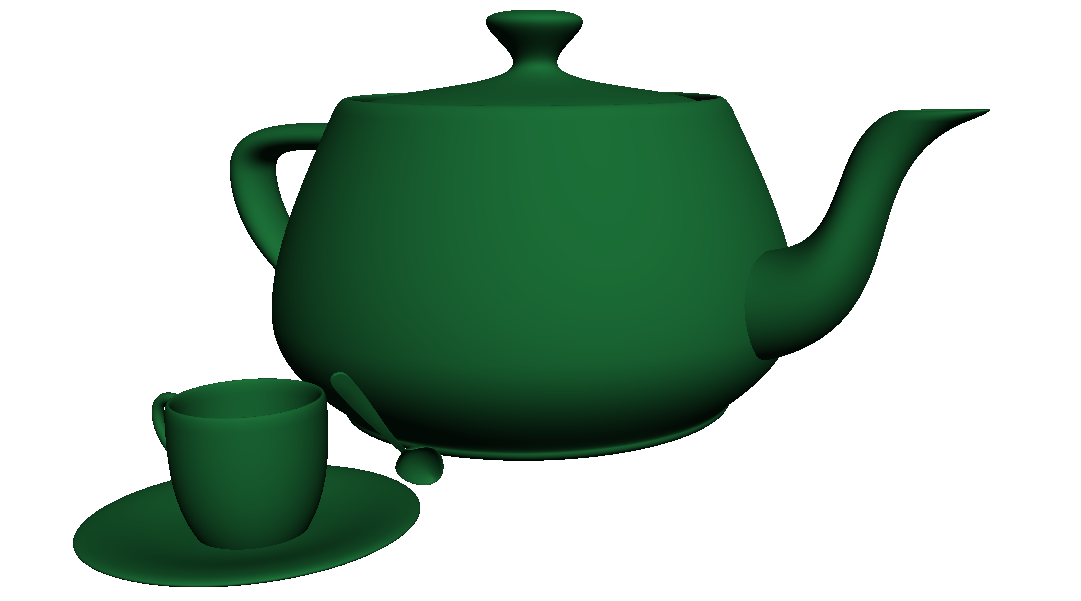
\includegraphics[width=0.2\textwidth]{"/home/lee/Desktop/CG/PA2/report/multi-Bezier_surface.png"}
	\end{figure}
	\item multi-B-Spline-surface with degree 3
	\begin{figure}[H]
		\centering
		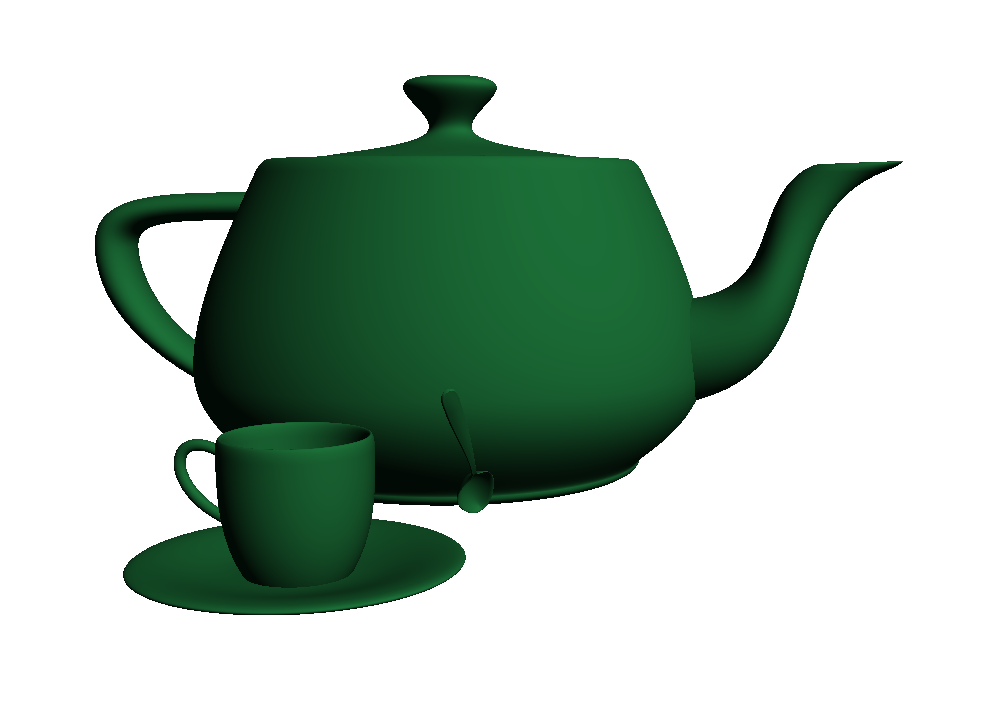
\includegraphics[width=0.2\textwidth]{"/home/lee/Desktop/CG/PA2/report/multi-B-spline-degree3.png"}
	\end{figure}
	\item multi-B-Spline-surface with degree 2
	\begin{figure}[H]
		\centering
		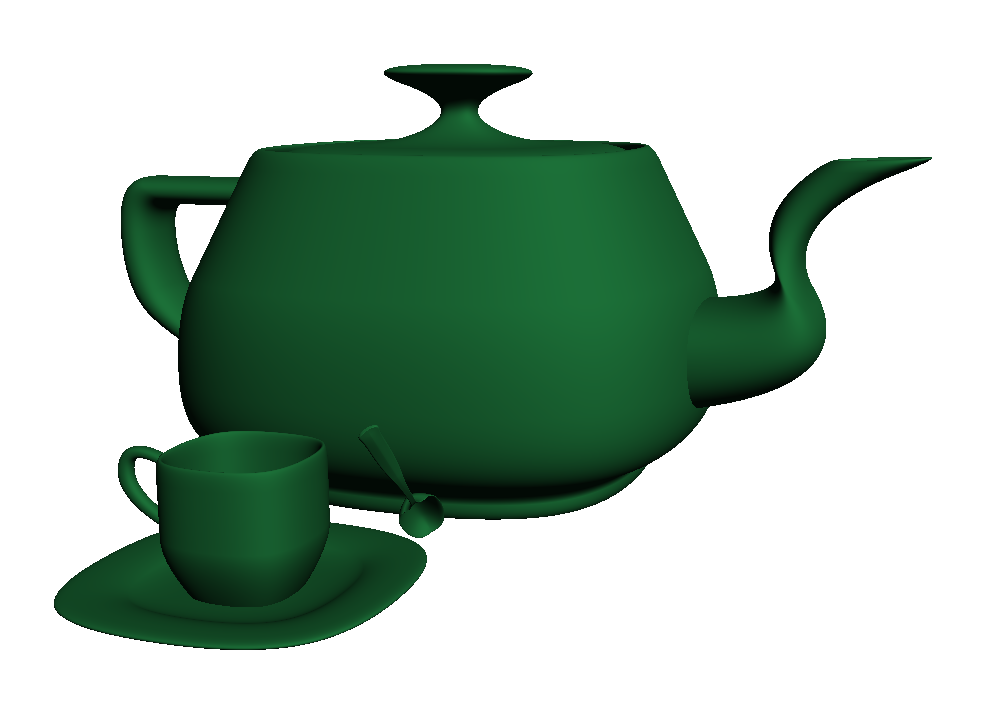
\includegraphics[width=0.2\textwidth]{"/home/lee/Desktop/CG/PA2/report/multi-B-spline-degree2.png"}
	\end{figure}
	\item multi-B-Spline-surface with degree 1
	\begin{figure}[H]
		\centering
		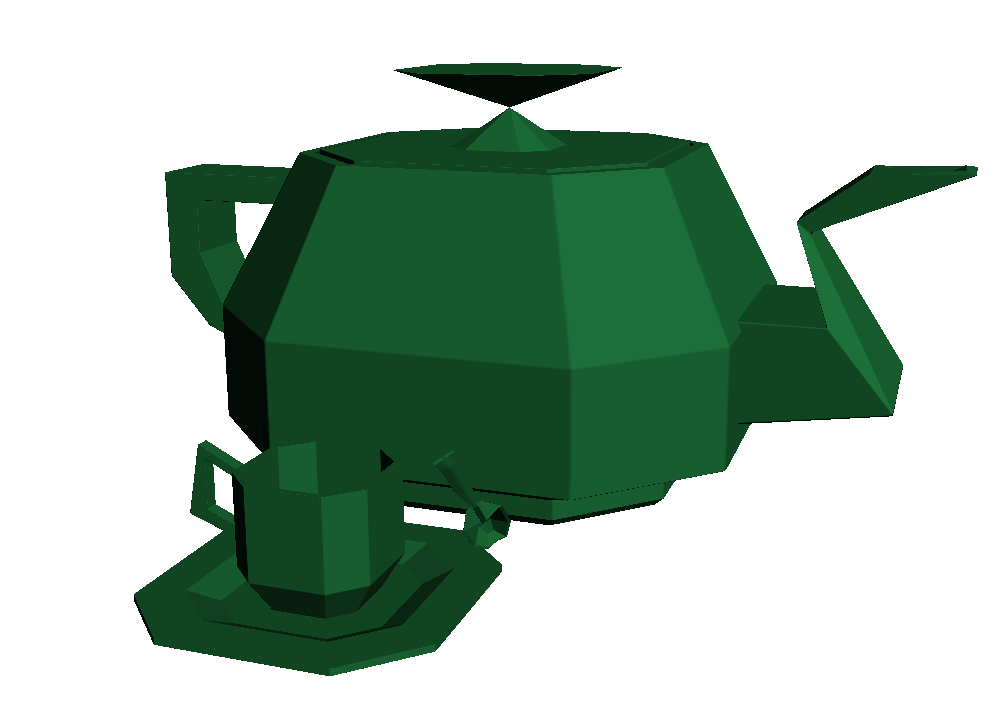
\includegraphics[width=0.2\textwidth]{"/home/lee/Desktop/CG/PA2/report/multi-B-spline-degree1.png"}
	\end{figure}
	\item adaptive-mesh
	\begin{figure}[H]
		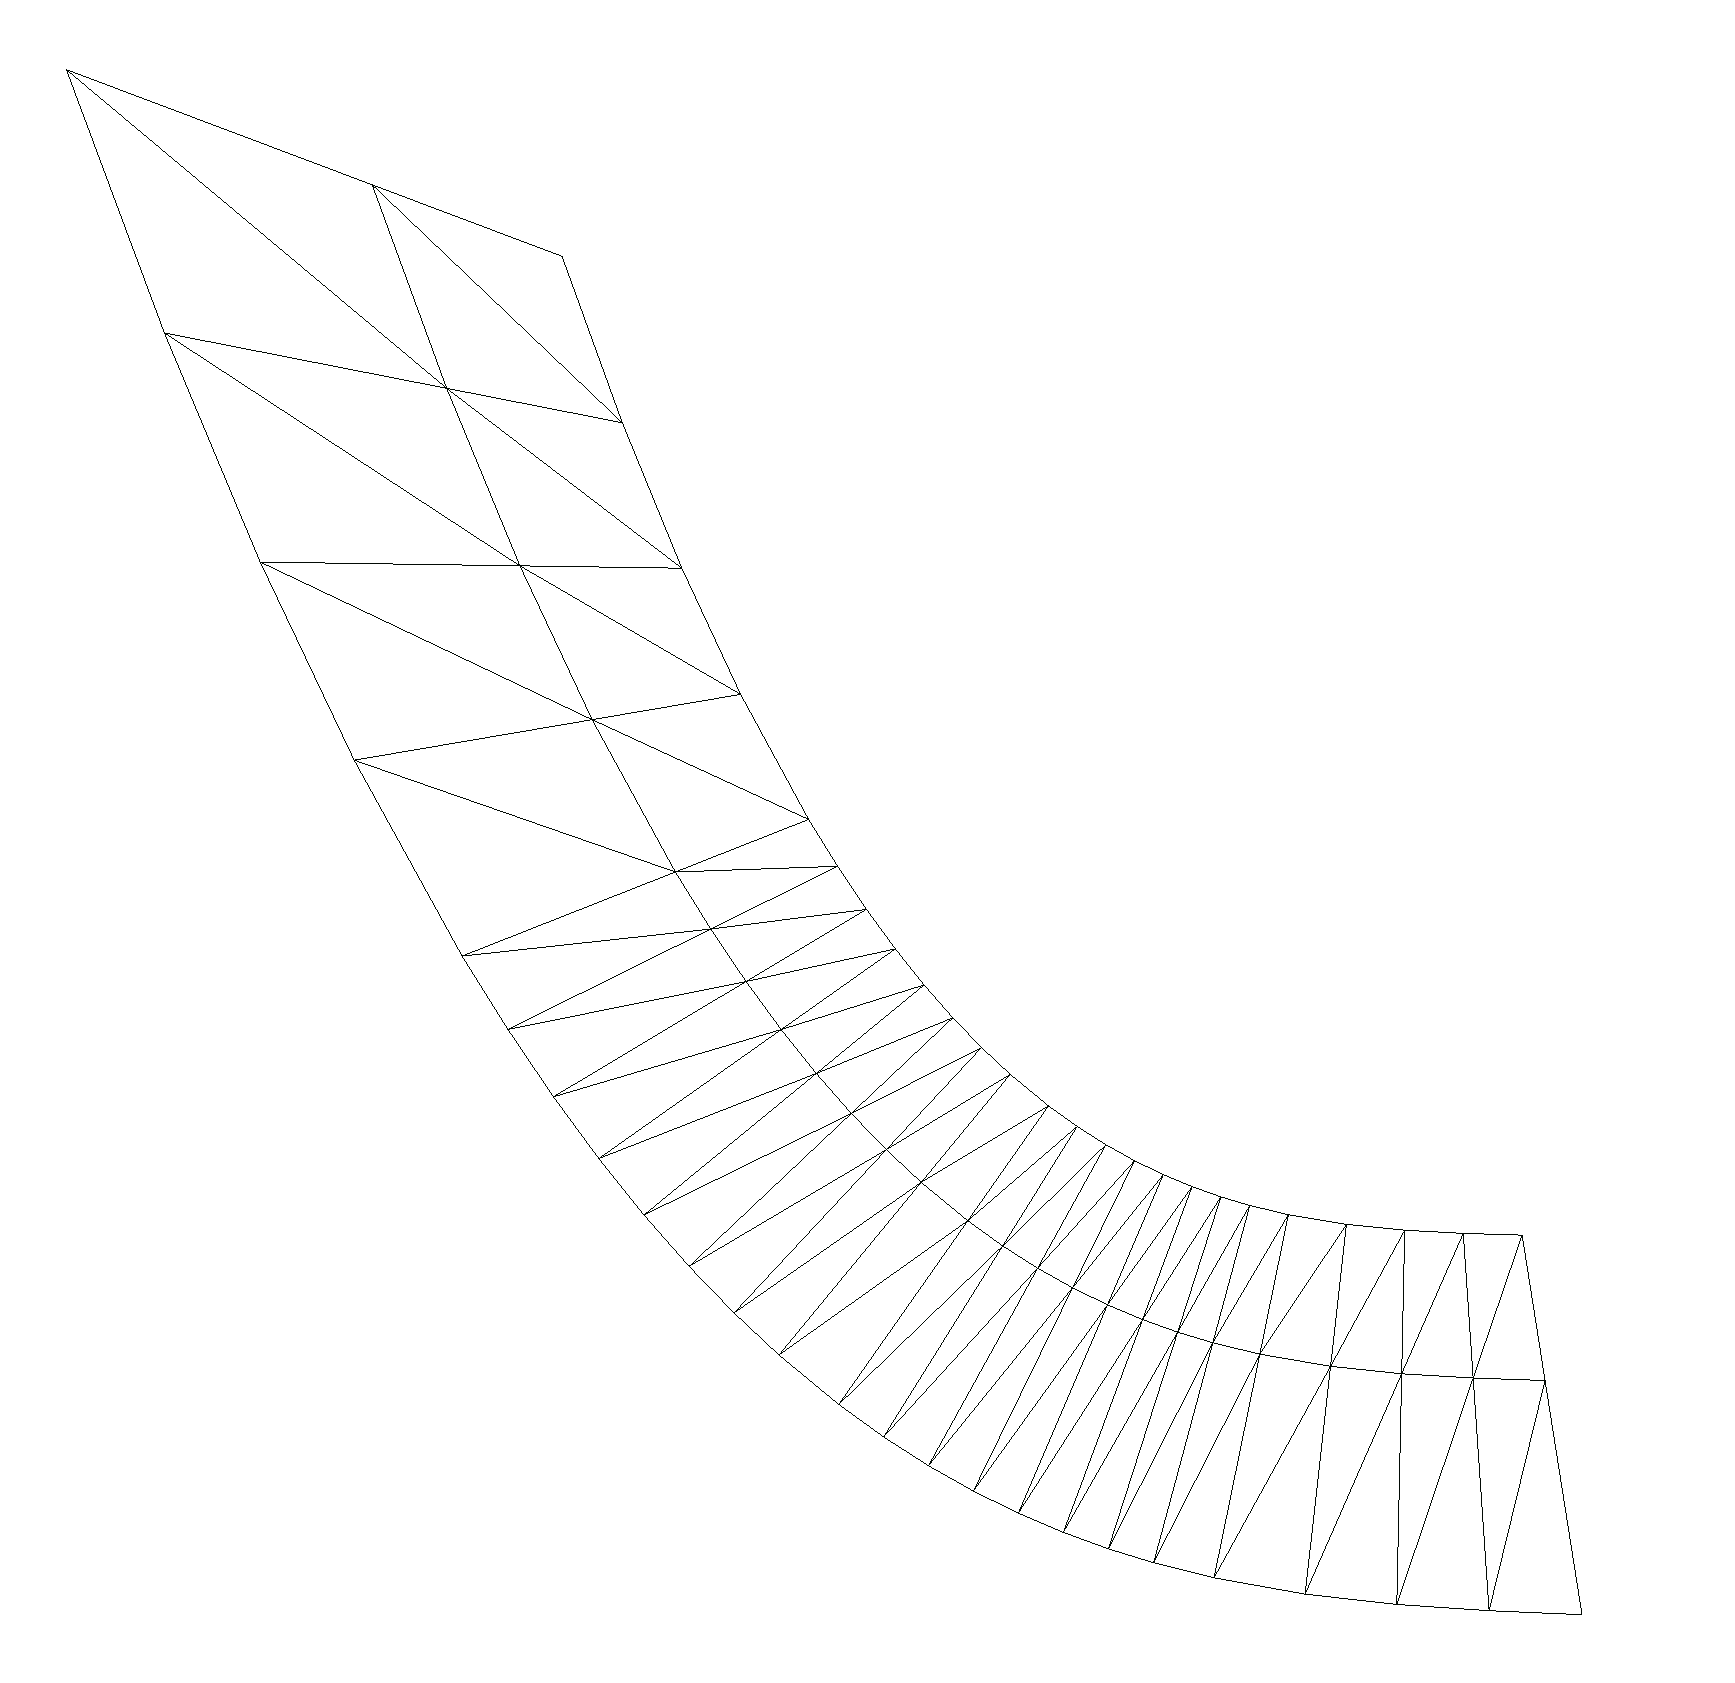
\includegraphics[width=0.2\textwidth]{"/home/lee/Desktop/CG/PA2/report/adaptive.png"}
		\caption{adaptive mesh}
		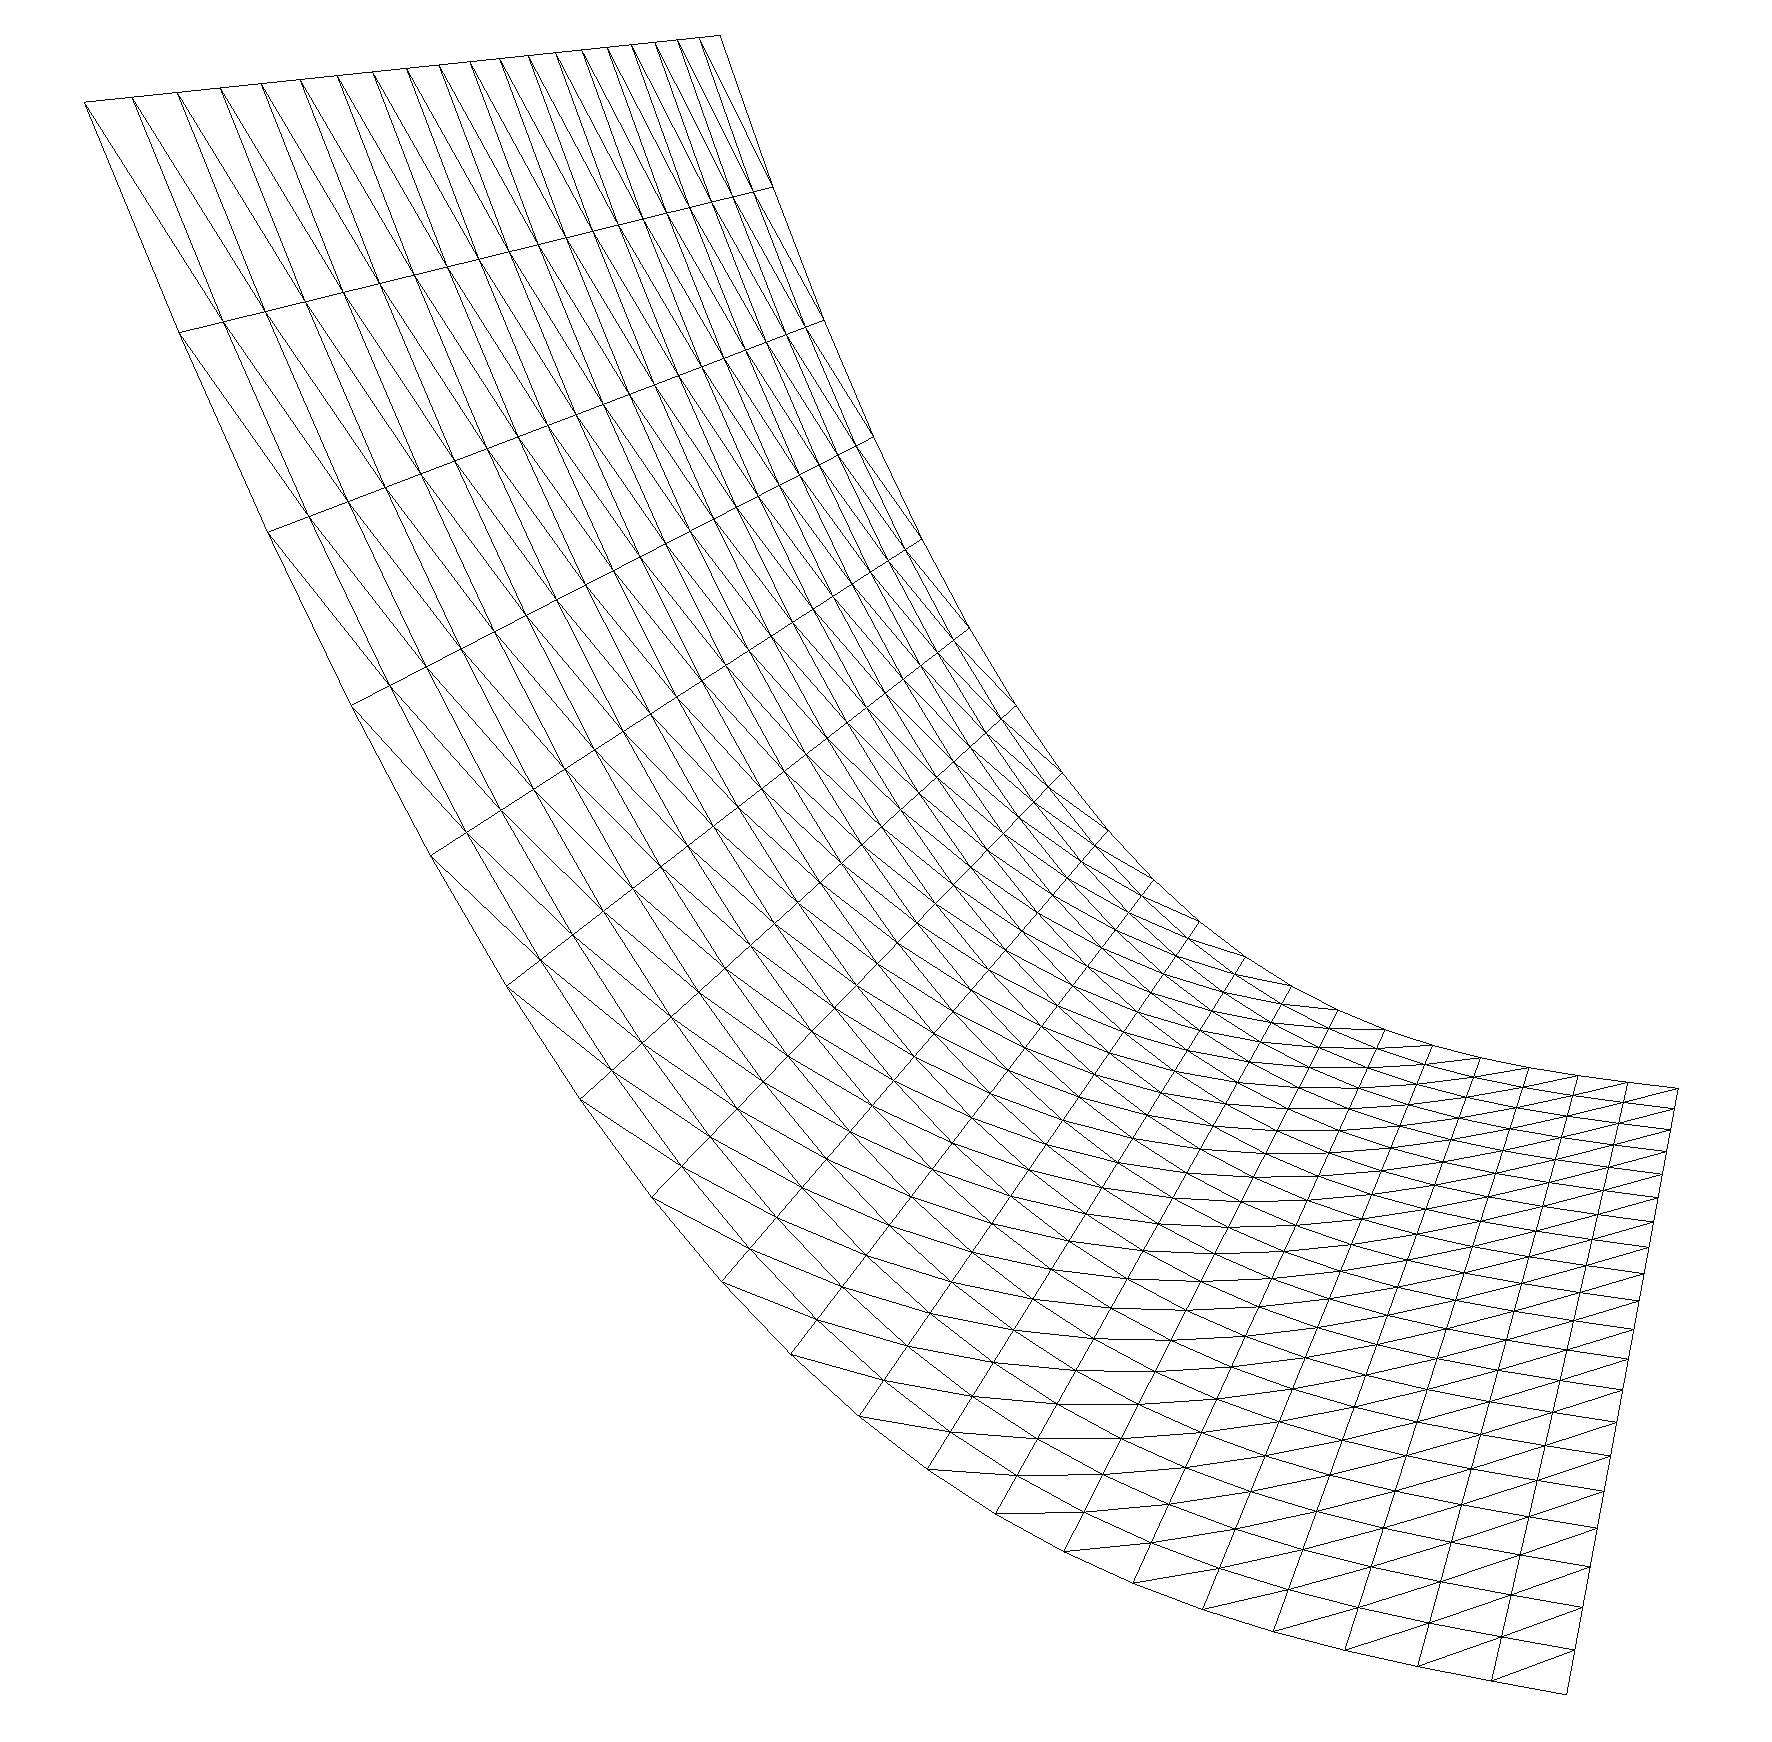
\includegraphics[width=0.2\textwidth]{"/home/lee/Desktop/CG/PA2/report/uniform.png"}
		\caption{uniform mesh}
	\end{figure}
\end{itemize}
% pictures should be in
\end{document}
